\documentclass[11pt]{article}
% Defining all packages that are used in this document
\usepackage[utf8]{inputenc}
\usepackage[english]{babel} % Change this to norwegian if report is written in norwegian
\usepackage{amsmath}   % Package for math files
\usepackage{parskip}   % No indent, but instead paragraphs
\usepackage{graphicx}  % Place figures
\usepackage{caption}   % Place captions in tables and figures
\usepackage{subcaption}% 
\usepackage{subfiles}  % 
%\usepackage{subfigure}
\usepackage{pdfpages}
\usepackage[T1]{fontenc} 
\usepackage[euler]{textgreek} % To get greek letters as we know them
\usepackage{amssymb}   % 
\usepackage{placeins}  % \FloatBarrier so figures can't float beyond some point in text
\usepackage{fullpage}  % Uses more of the page
\usepackage{float}     % Able to make figures and tables float \begin{figure}[H] to keep them HERE
\usepackage[version=4]{mhchem} % \ce{} to write chemical eq.
\usepackage{siunitx}   % Ex: \si{\meter\per\square\second}
\usepackage{booktabs}  % Behind-the-scenes optimization of tables. \toprule, \midrule, \bottomrule
\usepackage{hyperref}  % Ability to click on references like equations, figures, sections etc. \ref{eq:my_eq} clickable
\hypersetup{
    colorlinks,
    citecolor=black,
    filecolor=black,
    linkcolor=black,
    urlcolor=black
}
\usepackage{fancyhdr}
	%fancyhdr:一个很强大的宏包,用于自定义设计页面风格并命名以供调用。
	\pagestyle{fancy}
	%\rhead{实验B16 基于vLight的光学仿真基础实验}
	%\lhead{基础物理实验\uppercase\expandafter{\romannumeral2}实验报告}
	\cfoot{ \thepage}  %当前页
	\rfoot{\today}
		%分别是右页眉、左页眉、中页脚、右页脚
	\renewcommand{\headrulewidth}{0pt}
	\renewcommand{\theenumi}{(\arabic{enumi})}


\usepackage[autolinebreaks,useliterate,numbered]{mcode} % Ability to paste smooth MATLAB code
\newcommand{\figref}[1]{\figurename~\ref{#1}} %Nice reference to figures
%\linespread{1.5}
\renewcommand{\baselinestretch}{1.5}
\title{
    Lab Experiment \\
    Beam Bending
    }
\author{
	Jiaqi, Yao.\footnote{jy431@exeter.ac.uk}
}
\date{
    \today
}

\begin{document}
\maketitle
%\begin{abstract}
%    This section should contain a short and concise way of describing all parts of the report. It should be a summary of the introduction, what has been done and what you have found.
%\end{abstract}
\pagenumbering{gobble} % Turn off page numbering
%\newpage
%\tableofcontents
%\newpage
\pagenumbering{arabic} % Turn on normal pagenumbering
%%%%%%%%%%%%%%%%%%%%%%%%%%%%%%%%%%%%%%%%%%%%%%%%%%%%%%%%%%
% Main contents - Do NOT write your text in main.tex! Use                     the tex files in the folders below
\section*{Section A}
\label{sec:Section A}
\FloatBarrier % Now figures cannot float above section title


In this section, the Young's modulus of two materials 
(mild steel and aluminium) can be calculated from experimental data.

A total of six groups of data were obtained from the experiment. (See Table \ref{t1})

\subsection*{Analysis}

By plotting these 6 groups of data on a scatter plot and performing 
regression analysis, a total of 6 groups of graphs were obtained. (See Figure \ref{f1})

\begin{figure}
    \centering
    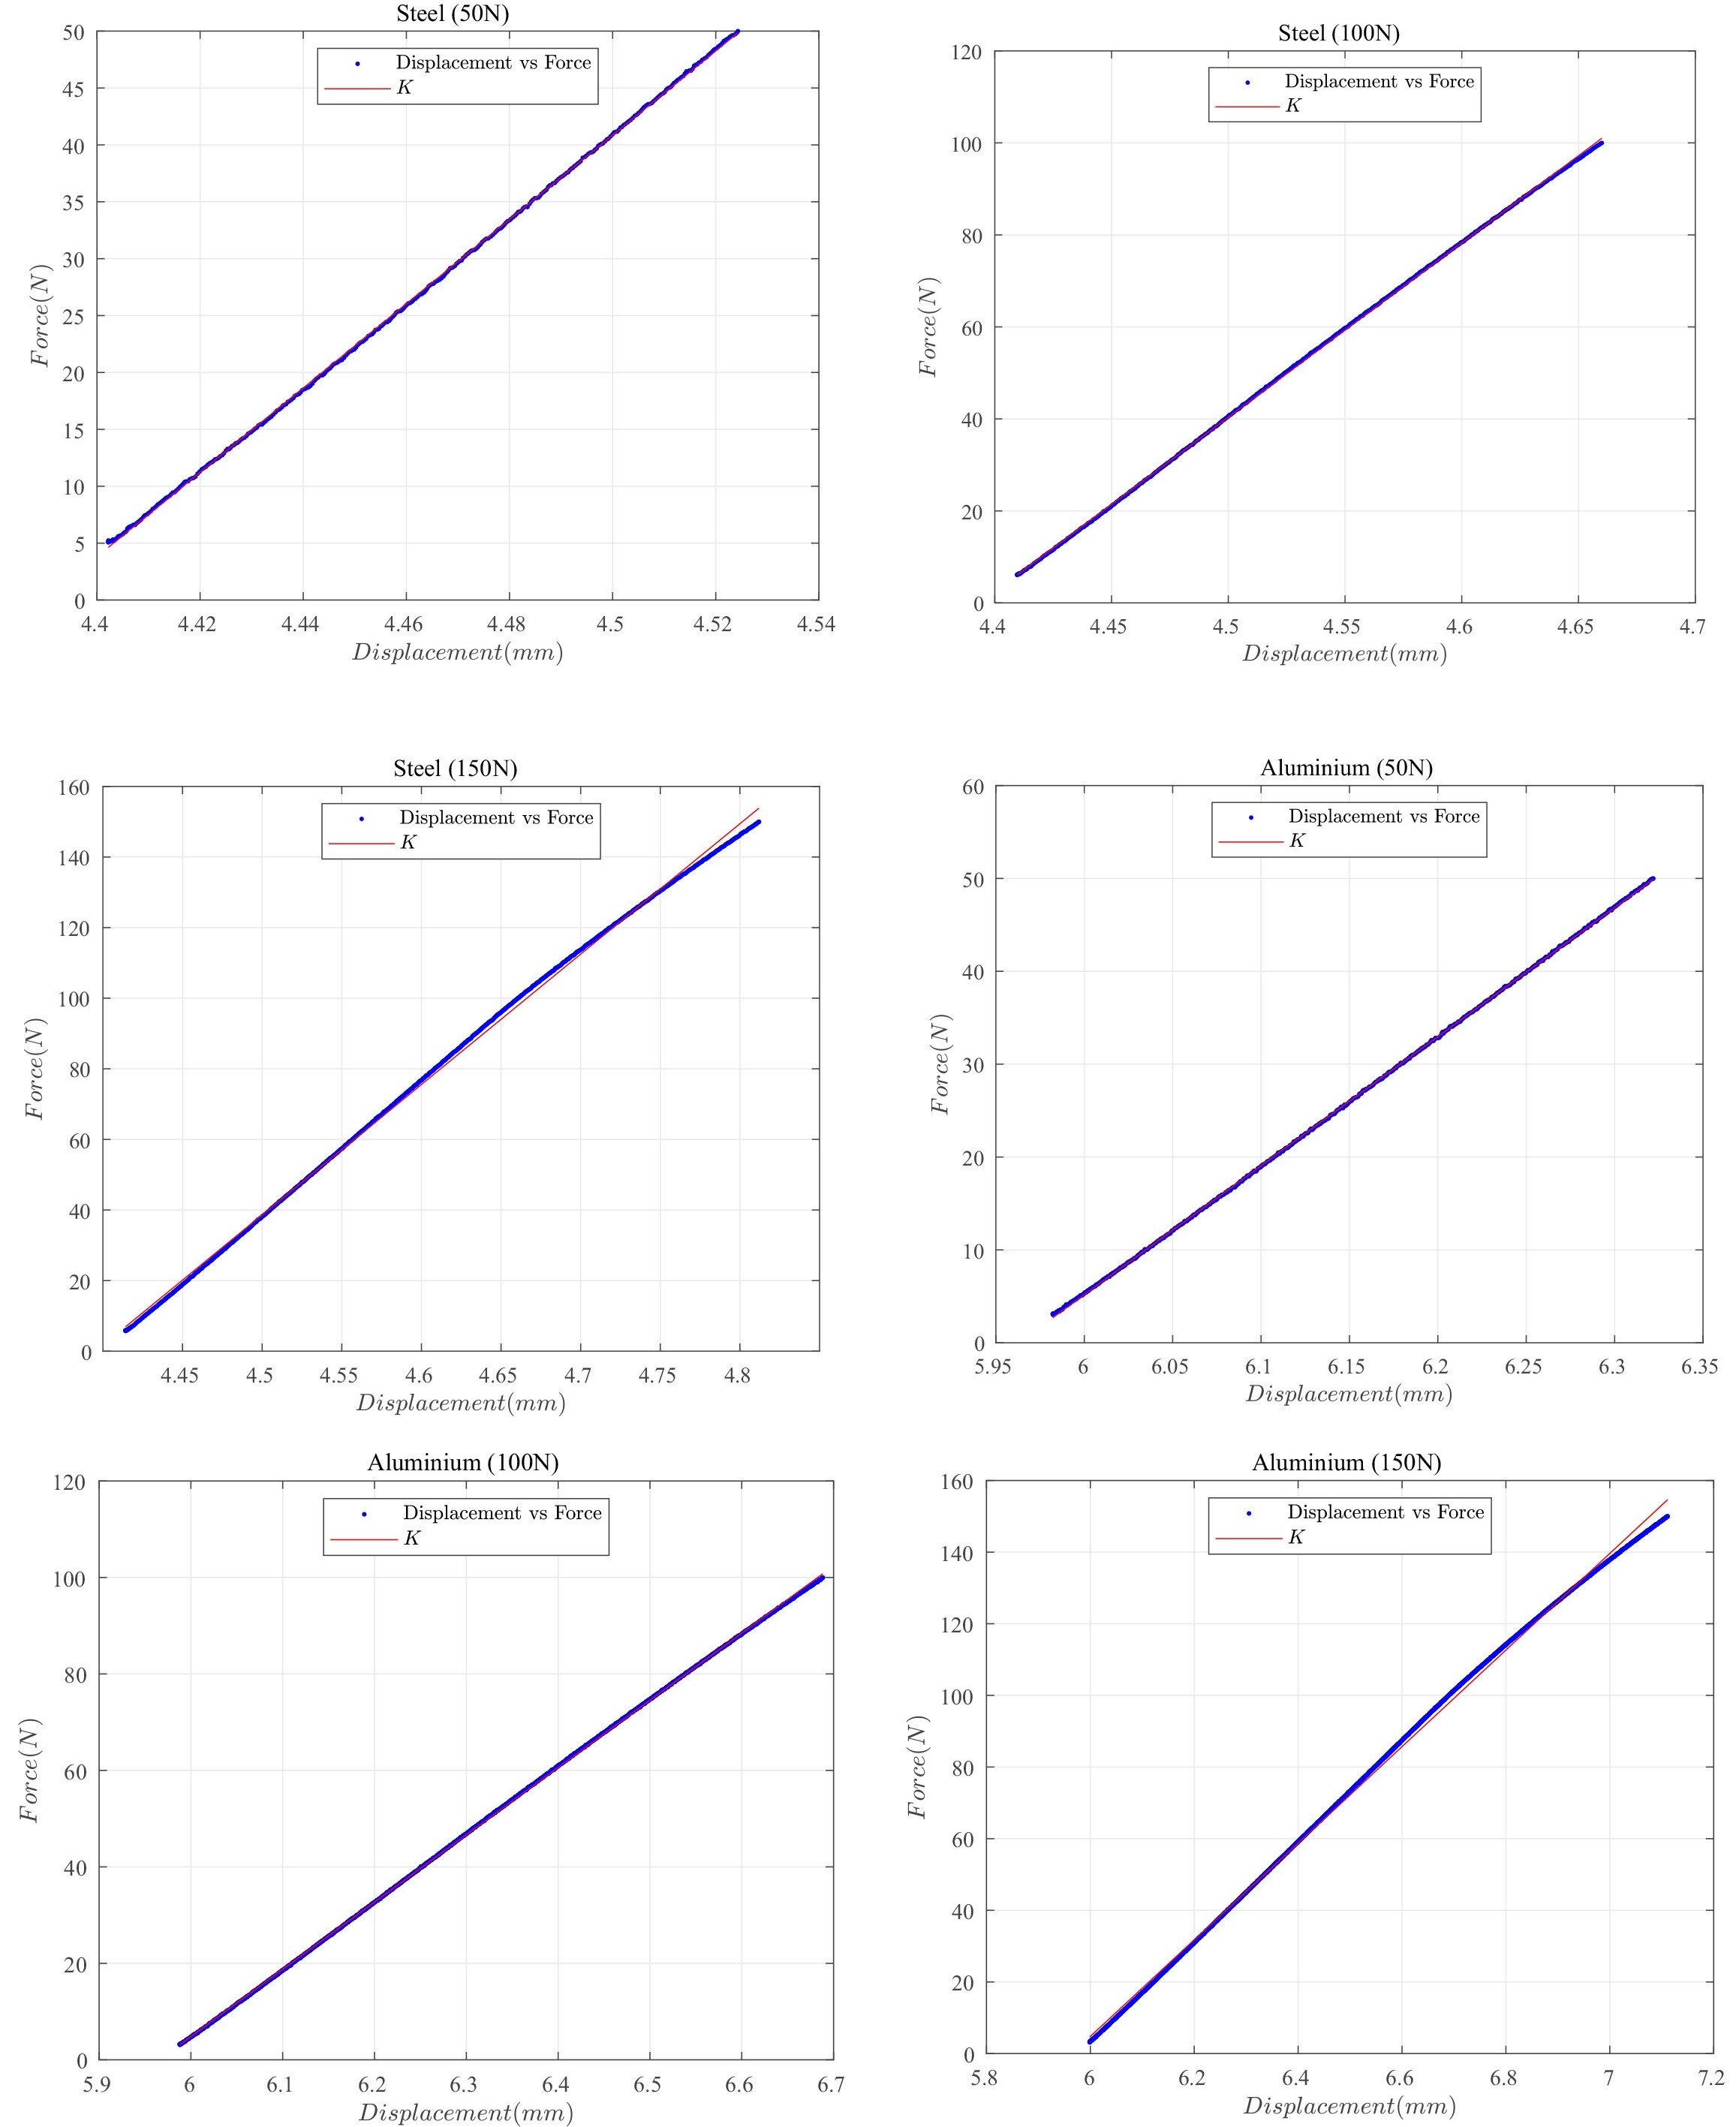
\includegraphics[width=15cm,height=21.5cm]{./fig/mix.jpg}
    \caption{Figure of linear regression analysis}
    \label{f1}
\end{figure}

\begin{minipage}[htbp]{\textwidth}
    \makeatletter\def\@captype{table}
    \centering
    \scalebox{1}{
    \begin{tabular}{lllll} 
        \hline
        No.  & Material    & Final load (N) &K(Slope)& R-square    \\ \hline
        1 & Steel     & 50   &370.4& 0.9999\\
        2 & Steel      & 100  &379.1& 0.9998\\
        3 & Steel      & 150   &369.4& 0.9989\\
        4 & Aluminium     & 50  &138.9& 0.9999\\
        5 & Aluminium    & 100   &139.4& 0.9999\\
        6 & Aluminium & 150   &134.8& 0.9987\\ \hline          
    \end{tabular}} 
    
    (Notice: The unit of K is N/mm, it needs to multiply $10^3$ to transfer to N/m)
    \caption{Experimental data and linear regression results}
    \label{t1} 
\end{minipage}

In order to calculate E, the moment of inertia I needs to be calculated first.

\begin{equation} 
I=\frac{bh^3}{12}=\frac{20*3^3}{12}*10^{-12}=4.5*10^{-11} (mm^4)
\end{equation}

We know 
\begin{equation} 
    \delta_{max}=\frac{PL^3}{48EI}
\end{equation}

And the slope of the regression analysis is
\begin{equation} 
    K=\frac{P}{\delta}=\frac{48EI}{L^3}
\end{equation}

So
\begin{equation} 
    E=(\frac{P}{\delta})*\frac{L^3}{48I}=K*\frac{L^3}{48I}
\end{equation}

Calculate each group of data and obtain the table \ref{t2}.

\begin{minipage}[htbp]{\textwidth}
    \makeatletter\def\@captype{table}
    \centering
    \scalebox{1.1}{
    \begin{tabular}{lll} 
        \hline
        Modulus of Elasticity  & Mild Steel    & Aluminium     \\ \hline
        $E_1(P=50N)$ & 171.482     & 64.3056    \\
        $E_2(P=100N)$ & 175.509     & 64.5370   \\
        $E_3(P=150N)$ & 171.019     & 62.4074   \\
        $E_{exp}=(E_1+E_2+E_3)/3$ & 172.670 & 63.75   \\ \hline          
    \end{tabular}} 
    
    (Unit: GPa)
    \caption{Experimental results - Modulus of elasticity}
    \label{t2} 
\end{minipage}


\subsection*{Summary}

As can be seen from the data in Table \ref{t2}, 
the modulus of elasticity of mild steel (172.67GPa) is much larger than aluminium (63.75GPa).
In addition, due to the difference in modulus of elasticity, the deformation of aluminium is 
greater than that of mild steel under the same force.

The comparison for each material indicates that there is a slight difference 
in the modulus of elasticity, 
which may be due to experimental error, and the more accurate 
modulus of elasticity can be obtained through more 
experiments.

\section*{Section B}
\label{sec:Section B}
\FloatBarrier % Now figures cannot float above section title
In this section, the deformation of each material under different 
forces can be calculated from the data obtained in section A.

\subsection*{Analysis}

We know
\begin{equation} 
    \delta_{max}=\frac{PL^3}{48EI}=\frac{P*0.1^3}{48*E_{exp}*4.5*10^{-11}}
\end{equation}

Using the $E_{exp}$ in different material(Mild Steel and Aluminium)
 with different force(50N, 100N, 150N) in Table \ref{t2}, the data in Table \ref{t3} can be calculated.

\begin{minipage}[htbp]{\textwidth}
    \makeatletter\def\@captype{table}
    \centering
    \scalebox{1.1}{
    \begin{tabular}{lll} 
        \hline
        Bending Displacement  & Mild Steel    & Aluminium     \\ \hline
        $\delta_{AN\_{1}}(P=50N)$ & 0.1341    & 0.3631    \\
        $\delta_{AN\_{2}}(P=100N)$ & 0.2681     & 0.7262   \\
        $\delta_{AN\_{3}}(P=150N)$ & 0.4022     & 1.0893  \\ \hline          
    \end{tabular}} 
    
    (Unit: mm)
    \caption{Experimental results - maximum deformation}
    \label{t3} 
\end{minipage}

\subsection*{Summary}

Bringing the average modulus of elasticity into the equation enables 
a more accurate calculation of the deformation of the material under 
different forces and helps to reduce experimental errors.
\section*{Section C}
\label{sec:Section C}
\FloatBarrier % Now figures cannot float above section title

In this section, finite element analysis (ANSYS) is performed on the components.

\subsection*{Analysis}

ANSYS analysis results are shown in Figure \ref{f2}.

\begin{figure}[htbp]
    \centering
    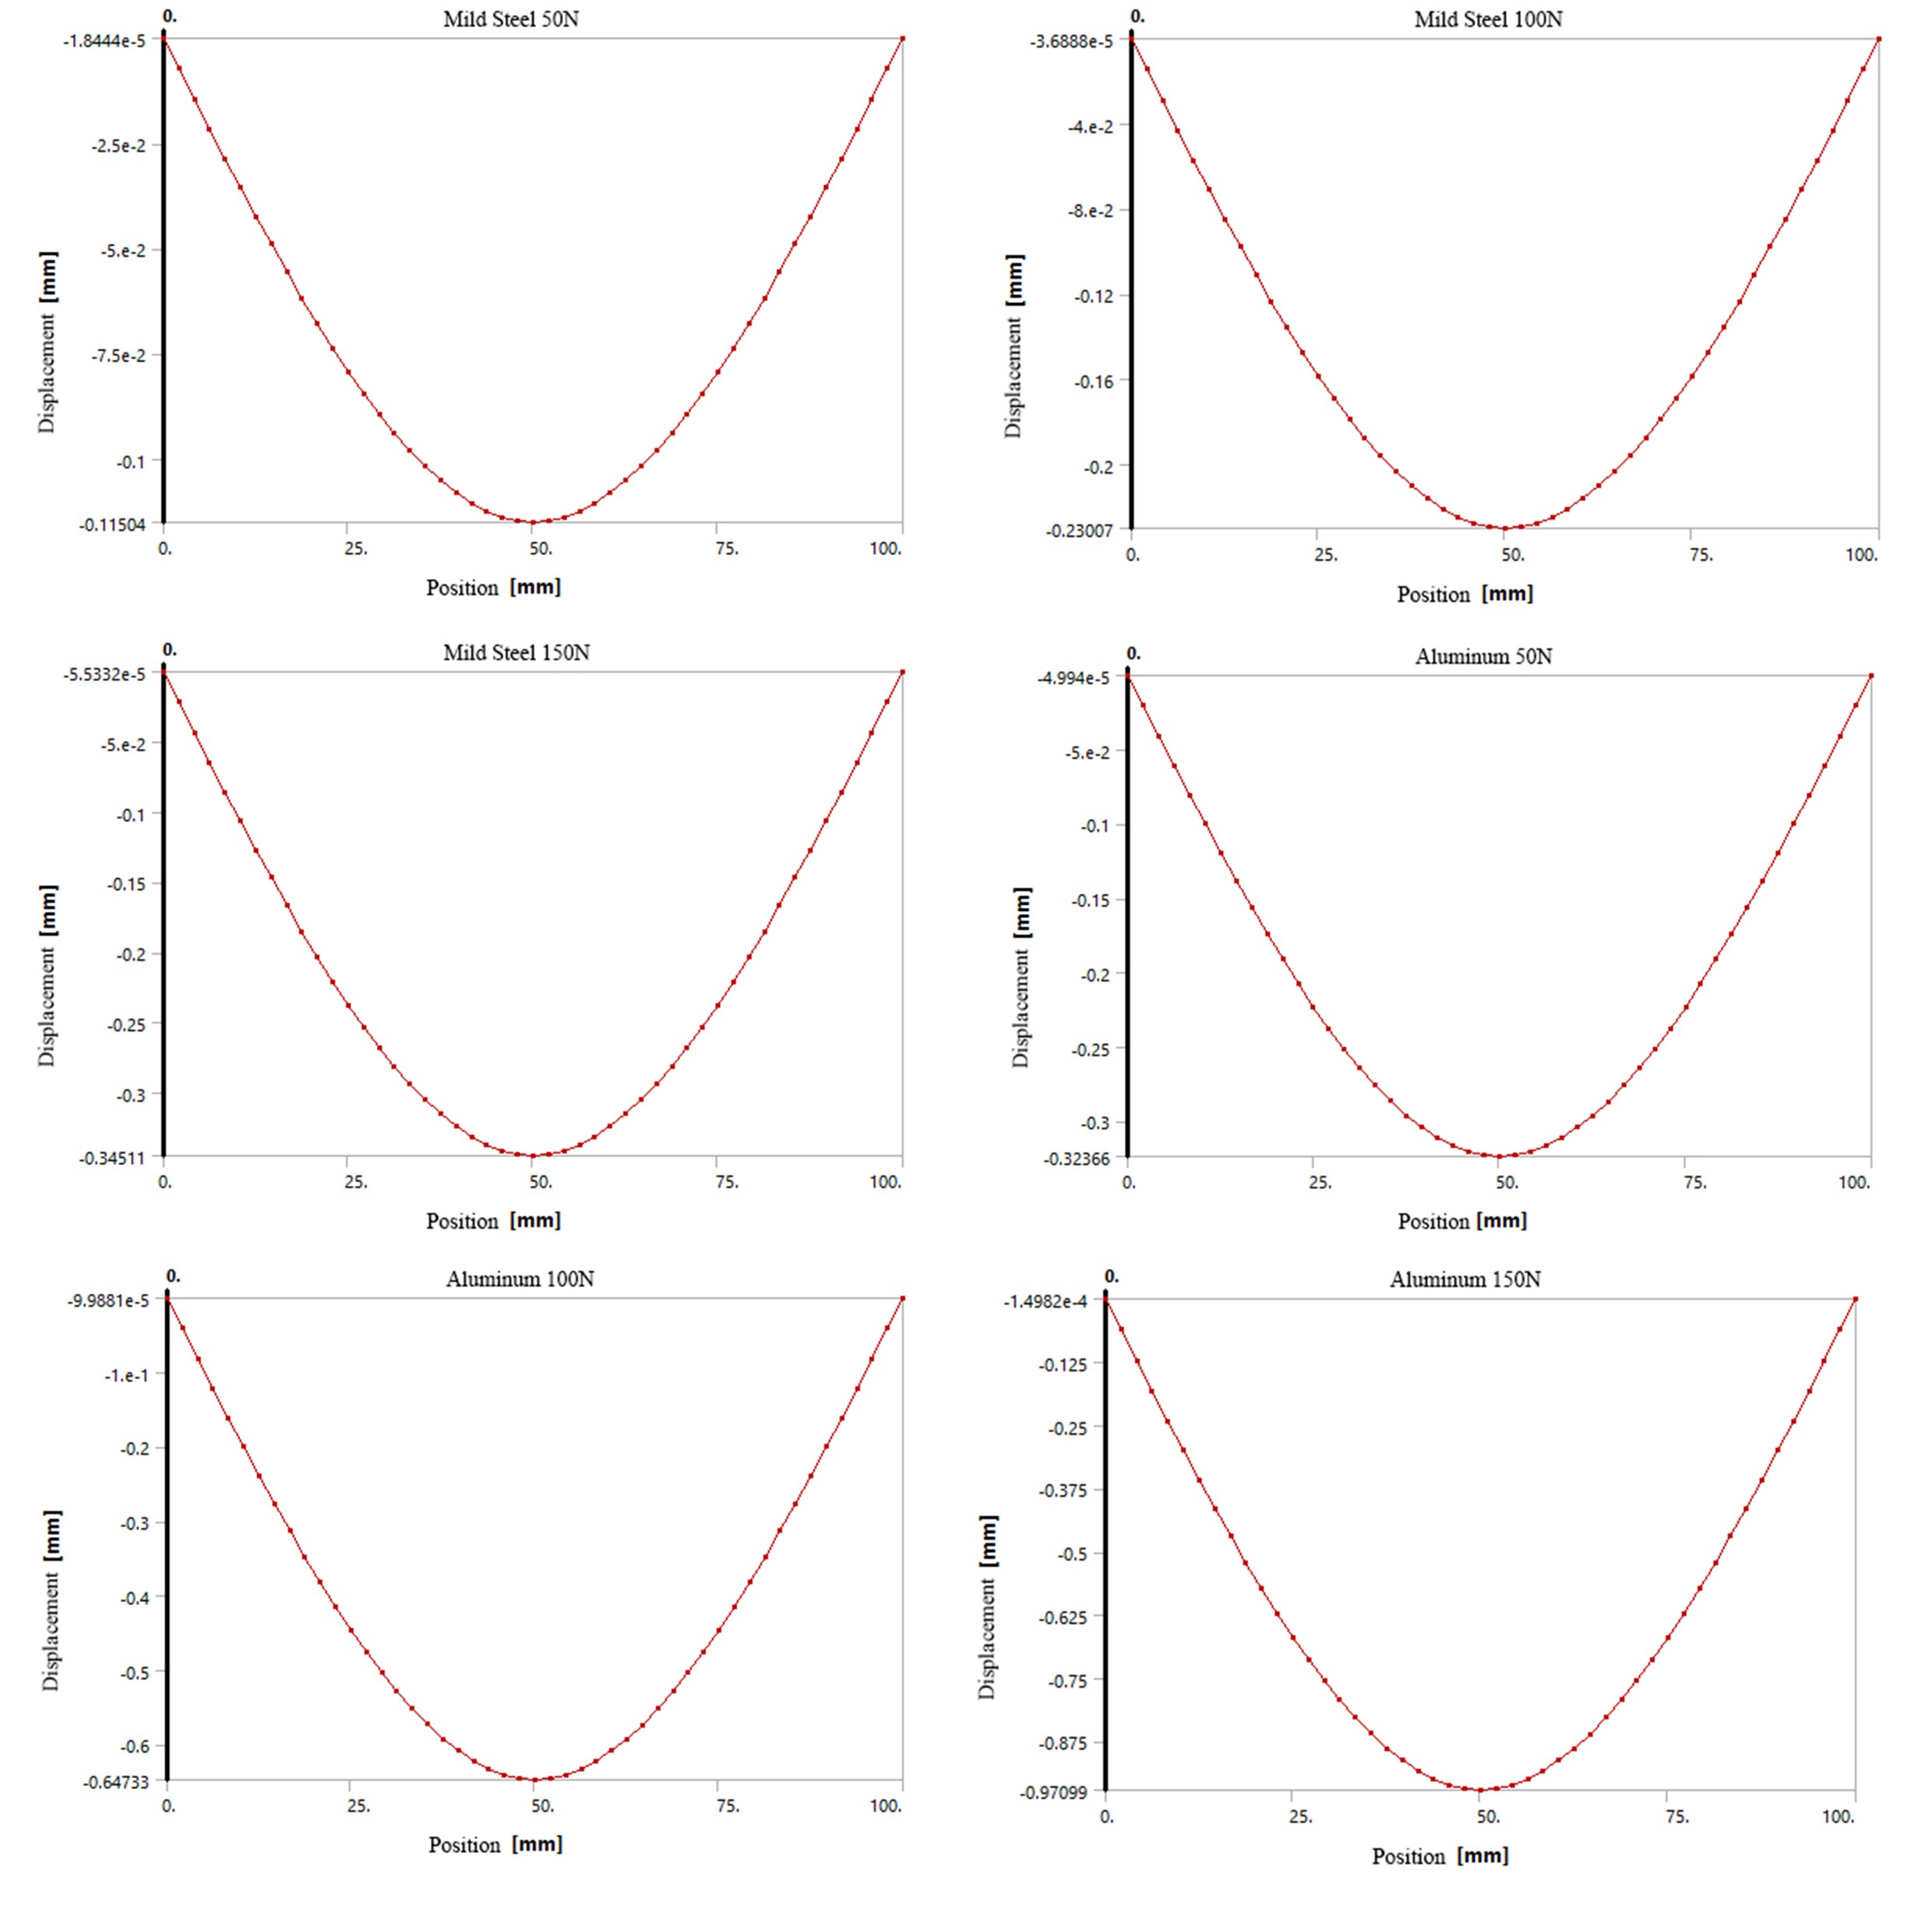
\includegraphics[width=18cm,height=20cm]{./fig/mix2.jpg}
    \caption{Figure of ANSYS analysis}
    \label{f2}
\end{figure}


The finite element analysis in Figure \ref{f2} gives the deformation-position 
curves for different materials under different forces, 
where the maximum deformation of the component can be easily determined.

The data are shown in Table \ref{t4}.

\begin{minipage}[htbp]{\textwidth}
    \makeatletter\def\@captype{table}
    \centering
    \scalebox{1.1}{
    \begin{tabular}{lll} 
        \hline
        Bending Displacement  & Mild Steel    & Aluminium     \\ \hline
        $\delta_{FE\_{1}}(P=50N)$ & 0.1150    & 0.3237    \\
        $\delta_{FE\_{2}}(P=100N)$ & 0.2300    & 0.6473  \\
        $\delta_{FE\_{3}}(P=150N)$ & 0.3451    & 0.9710  \\ \hline          
    \end{tabular}} 
    
    (Unit: mm)
    \caption{FEA results - maximum deformation}
    \label{t4} 
\end{minipage}



\subsection*{Summary}
By using ANSYS analysis, deformation-displacement diagrams were obtained 
for two materials under three different forces, revealing that the maximum 
deformation exists at the midpoint of the element (the point where the forces are applied).

The comparison also shows that even under theoretical conditions, the deformation of aluminium \
is larger than that of mild steel under the same forces.
\section*{Section D}
\label{sec:Section D}
\FloatBarrier % Now figures cannot float above section title


\subsection*{Comparison of results}

By comparing the experimental data with the results of the ANSYS analysis, 
it can be found that all six groups of data measured in the laboratory have 
larger deformation values than the ANSYS analysis. This is due to the fact 
that the modulus of elasticity of the laboratory material is 172.67GPa(Mild Steel) and 63.75GPa(Aluminium), 
both of which are smaller than the theoretical value of the material(210GPa and 70GPa).


In addition, the percentage deformation of mild steel is larger than 
that of aluminium 
(i.e. $\frac{\delta_{AN}-\delta_{FE}}{\delta_{FE}}*100\%$)
and this may also be due to the larger modulus of elasticity of mild steel.

\subsection*{Possible reasons}
$\bullet$ Insufficient material purity or inhomogeneous density 
resulting in a modulus of elasticity less than the theoretical value.

$\bullet$ The memory effect of the metal caused by repeated use of the original 
experimental piece resulted in inaccurate deformation of the measurement.

$\bullet$ Errors caused by machines not being calibrated before measurement or 
by the machine's own measurement issues.

\subsection*{Experimental improvements}

$\bullet$ Replacement of materials with new materials which are not affected by 
the memory effects.

$\bullet$ Choose higher purity and more homogeneous density with higher precision 
components for measurement.

$\bullet$ Change the machine and take several measurements to avoid experimental chance.

%\section*{List of Symbols}
\begin{table}[H]
\centering
\begin{tabular}{lll}
 \toprule
  \textbf{Symbol}   &\textbf{Unit}      &\textbf{Explanation}\\
  \midrule
    n               & \si{\mole}        & Amount of substance \\
    m               & \si{\kilo\gram}   & Mass \\
    H               & \si{\kilo\joule\per\mole} & Molar enthalpy \\
    S               & \si{\joule\per\kelvin\per\mole}   & Molar entropy \\
    G               & \si{\kilo\joule\per\mole} & Gibbs free energy \\
    A               & \si{\kilo\joule\per\mole} & Helmholtz free energy \\
  \bottomrule
  \end{tabular}
\end{table}

%%%%%%%%%%%%%%%%%%%%%%%%%%%%%%%%%%%%%%%%%%%%%%%%%%%%%%%%%%
% Bibliography
\newpage
\bibliographystyle{IEEEtran}
\bibliography{mendeley.bib}
%%%%%%%%%%%%%%%%%%%%%%%%%%%%%%%%%%%%%%%%%%%%%%%%%%%%%%%%%%
% Appendix
%\appendix
%\pagenumbering{roman}
%\section{First Appendix}
\label{app:first_appendix}
%\section{Second Appendix}
%\section{Third Appendix}
\end{document}
